\section{Описание проекта}
\subsection{Авторизация}
Авторизация --- это процесс предоставления определённому лицу или группе лиц прав на выполнение определённых действий. Также сюда входит проверка данных, прав при попытке выполнения этих действий.

\subsection{Аутентификация}
Аутентификация --- процедура проверки подлинности.

\subsubsection{\acrfull{jwt}}
\begin{figure}[h!]
    \begin{center}
        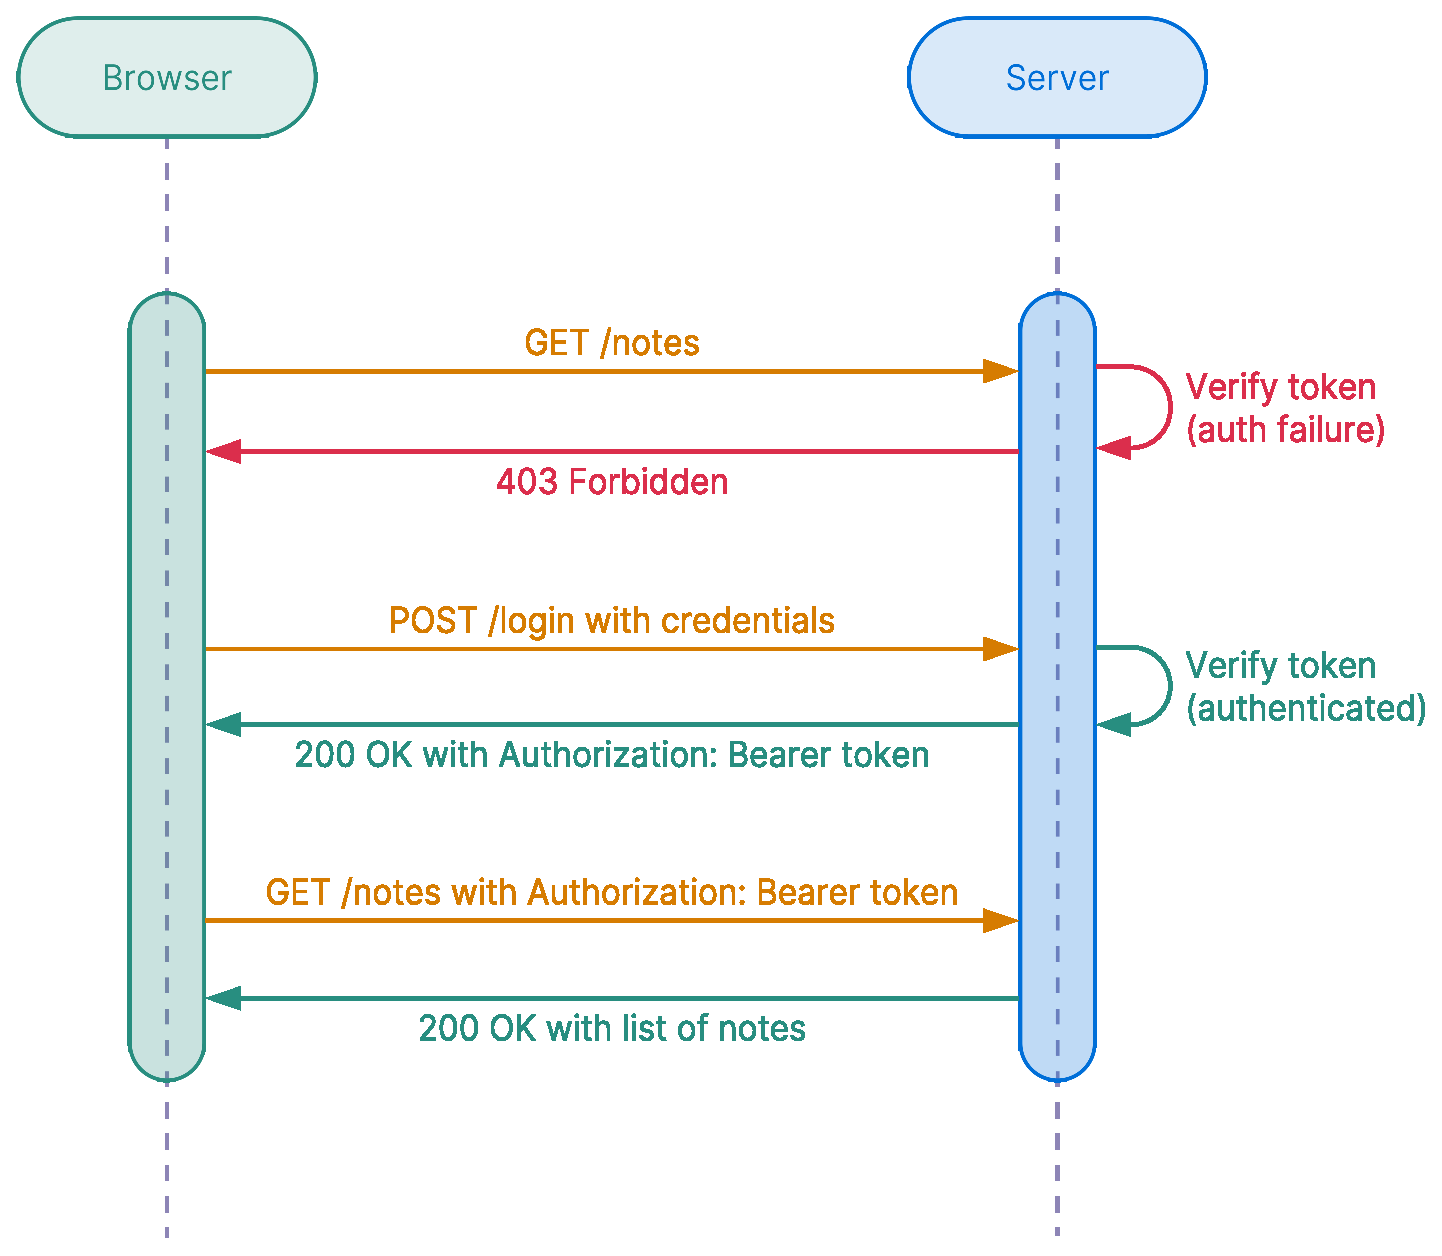
\includegraphics[scale=0.4]{images/jwt-example.eps}
        \caption{Демонстрация работы \acrshort{jwt}}
    \end{center}
\end{figure}

\acrfull{jwt} --- это открытый стандарт \href{https://tools.ietf.org/html/rfc7519}{(RFC 7519)}, который определяет способ для безопасной передачи информации между сторонами с помощью \acrshort{json} объектов. Эту информацию можно проверить, потому что она имеет цифровую подпись.

Вот несколько сценариев, в которых полезен \acrshort{jwt}:
\begin{itemize}
    \item Авторизация --- это наиболее распространенный сценарий использования \acrshort{jwt}. После того, как пользователь вошел в систему, каждый последующий запрос будет включать \acrshort{jwt}, позволяя пользователю получать доступ к маршрутам, службам и ресурсам, разрешенным с помощью этого токена.
    \item Обмен информацией --- \acrshort{jwt} хороший способ безопасной передачи информации между сторонами. Поскольку \acrshort{jwt} могут быть подписаны, например, с использованием пар открытого и закрытого ключей, вы можете быть уверены, что отправители являются теми, кем они себя называют. Кроме того, поскольку подпись рассчитывается с использованием \textbf{заголовка} и \textbf{полезных данных}, вы также можете убедиться, что содержимое не было изменено.
\end{itemize}

\clearpage